\documentclass[conference,a4paper]{IEEEtran}

\usepackage[utf8]{inputenc}
\usepackage[T1]{fontenc}
\usepackage[spanish,es-tabla,es-nodecimaldot,es-noshorthands]{babel}
\usepackage{graphicx}
\usepackage{booktabs}
\usepackage{amsmath}
\usepackage{listings}
\usepackage{xcolor}
\usepackage{url}
\usepackage[hidelinks]{hyperref}

\renewcommand\IEEEkeywordsname{Palabras clave}
\graphicspath{{figuras/}}

\lstset{language=Python, basicstyle=\ttfamily\scriptsize, columns=fullflexible,
  keepspaces=true, frame=single, rulecolor=\color{gray!50},
  commentstyle=\color{gray}, keywordstyle=\bfseries, showstringspaces=false,
  aboveskip=4pt, belowskip=4pt}

\begin{document}

\title{Accidentes bus--moto y despacho de ambulancias en Cuenca: un gemelo digital con SUMO y TraCI}

\author{\IEEEauthorblockN{Fernando Terán}
\IEEEauthorblockA{Redes Vehiculares y Heterogéneas\\
Universidad de Cuenca\\
fernandoj.teran@ucuenca.edu.ec}
\and
\IEEEauthorblockN{Docente: Pablo Barbecho}
\IEEEauthorblockA{Práctica 4 --- Reto de ambulancias\\
Cuenca, 28 de octubre de 2026}}

\maketitle

\begin{abstract}
Se construyó un gemelo digital del tráfico de Cuenca con SUMO~1.28 sobre las vías
arteriales de OpenStreetMap, con tres clases de vehículos de fondo (auto, bus y moto) y
siete hospitales. Mediante TraCI se provocan cinco accidentes bus--moto por hora durante
tres horas, desactivando el término de velocidad segura del modelo de Krauss en una moto
que alcanza a un bus. Cada accidente se detecta, se inmoviliza y se atiende con una
ambulancia despachada desde el hospital con menor tiempo de viaje que tenga una unidad
disponible, con una probabilidad de negativa $p_{\mathrm{sin}}=0{,}25$; tras la atención,
la ambulancia vuelve al hospital más cercano al accidente. En la corrida de referencia se
registraron 15 accidentes en 15 lugares distintos, sin teletransportes; la mediana del
tiempo de respuesta fue de 265~s y su percentil 90 de 354~s, ningún accidente esperó por
falta de ambulancia y el 47\,\% de los retornos terminó en un hospital distinto del de
origen. La comparación con la política de retorno al hospital de origen muestra que
volver al hospital más cercano acorta las misiones y la cola de la distribución de
respuestas, a costa de redistribuir la flota.
\end{abstract}

\begin{IEEEkeywords}
SUMO, TraCI, modelo de Krauss, gemelo digital, ambulancias, accidentes de tráfico.
\end{IEEEkeywords}

% ===========================================================================
\section{Introducción}
% ===========================================================================
Un accidente en una vía arterial afecta a dos sistemas a la vez: bloquea el tráfico y
consume recursos de emergencia que deben llegar a través de ese mismo tráfico. Los
simuladores microscópicos como SUMO~\cite{sumo} permiten estudiar esta interacción, pero
sus modelos de seguimiento están diseñados para no chocar. Esta práctica usa la interfaz
TraCI~\cite{traci} para romper deliberadamente esa garantía, provocar colisiones
controladas entre un bus y una moto, y gestionar la respuesta de una flota de ambulancias
repartida en siete hospitales de Cuenca.

El trabajo se organizó en seis fases: preparación del entorno (fase 0), construcción del
escenario y de la demanda (fase 1), hospitales y flota (fase 2), accidentes provocados
(fase 3), despacho, atención y retorno (fase 4) y estadísticas (fase 5). Además se
evaluó una política alternativa de retorno de las ambulancias.

% ===========================================================================
\section{Marco teórico}
% ===========================================================================
\subsection{Modelo de Krauss}
En cada paso $\Delta t$, el modelo de Krauss~\cite{krauss} toma la velocidad deseada
como el mínimo de tres términos y luego le resta una imperfección aleatoria:
\begin{align}
v_{\mathrm{des}} &= \min\left(v_{\mathrm{safe}},\; v_{\max},\; v + a\,\Delta t\right),\\
v &\leftarrow \max\!\left(0,\; v_{\mathrm{des}} - \sigma\, a\, \Delta t\, \eta\right),
\end{align}
donde $\eta\sim U(0,1)$ y $v_{\mathrm{safe}}$ es la mayor velocidad que permite detenerse
detrás del líder con la desaceleración $b$ si este frena, considerando el tiempo de
reacción $\tau$. Mientras el término $v_{\mathrm{safe}}$ participe en el mínimo, un
vehículo nunca embiste a su líder: la colisión es imposible por construcción.

\subsection{Control externo con TraCI}
\texttt{setSpeed(v)} solo fija $v_{\max}$ en la regla anterior; el mínimo sigue
aplicándose y el vehículo continúa frenando ante su líder. El comportamiento lo
determina la máscara de bits \texttt{setSpeedMode}: el bit~0 activa $v_{\mathrm{safe}}$,
el bit~1 limita la aceleración, el bit~2 limita la desaceleración, el bit~3 respeta la
prioridad en los cruces y el bit~4 respeta los semáforos en rojo. El valor por defecto
es 31 (todos los bits). Análogamente, \texttt{setLaneChangeMode} controla el modelo de
cambio de carril LC2013, cuyo valor por defecto es 1621.

% ===========================================================================
\section{Escenario}
% ===========================================================================
\subsection{Red vial}
El recuadro de lon $[-79{,}030;\,-78{,}950]$ y lat $[-2{,}930;\,-2{,}860]$ se descargó de
OpenStreetMap~\cite{osm} en $5\times5$ teselas (la API limita el número de nodos por
petición). Con \texttt{netconvert} se conservaron solo las vías \emph{tertiary} o
superiores (y sus enlaces), se unieron los cruces a menos de 25~m, se infirieron los
semáforos y se prohibieron los giros en U salvo en calles sin salida. Después se podaron
48 aristas en callejones sin salida con \texttt{prune\_deadends.py}. La red final,
\texttt{cuenca\_ciudad.net.xml}, tiene 1501 aristas (3955 contando las internas) y 98
semáforos; 1451 aristas pertenecen a la mayor componente fuertemente conexa y los siete
hospitales son alcanzables entre sí.

\subsection{Tipos de vehículo y demanda}
La Tabla~\ref{tab:vtypes} resume los tipos definidos en \texttt{vtypes.add.xml}. Los
valores del auto son los predeterminados de SUMO~\cite{vtypedef}; el bus es más lento en
aceleración y más regular ($\sigma$ menor), la moto es más agresiva ($\sigma=0{,}6$,
\texttt{speedFactor} 1,1) y la ambulancia conduce con poca imperfección y un
\texttt{speedFactor} de 1,3 que modela que excede el límite de velocidad.

\begin{table}[!t]
\centering
\caption{Tipos de vehículo (modelo de Krauss en todos)}
\label{tab:vtypes}
\footnotesize
\begin{tabular}{@{}lrrrrrrl@{}}
\toprule
Tipo & $L$ (m) & minGap & $a$ & $b$ & $\sigma$ & $\tau$ & Otros \\
\midrule
car       & 5,0  & 2,5 & 2,6 & 4,5 & 0,5 & 1,0 & --- \\
bus       & 12,0 & 3,0 & 1,2 & 4,0 & 0,3 & 1,2 & $v_{\max}=22$ \\
moto      & 2,2  & 1,0 & 3,5 & 6,0 & 0,6 & 1,0 & sF 1,1 \\
ambulance & 6,5  & 2,5 & 2,6 & 4,5 & 0,2 & 1,0 & sF 1,3 \\
\bottomrule
\end{tabular}
\end{table}

La demanda de fondo se generó con \texttt{randomTrips.py} (semilla 42,
\texttt{--validate}) durante 3~h: un auto cada 3~s (3600), un bus cada 36~s (300) y una
moto cada 12~s (900). La simulación dura 3,5~h para que la red se vacíe.

\subsection{Configuración de la simulación}
El archivo \texttt{reto.sumocfg} usa un paso de 1~s y fija tres opciones que son
condición para medir correctamente:
\begin{itemize}
\item \texttt{time-to-teleport = -1}: ningún vehículo atascado se teletransporta, de modo
que la cola detrás de un accidente persiste y se mide.
\item \texttt{collision.action = warn} con \texttt{collision.check-junctions} y
\texttt{mingap-factor = 0}: las colisiones se registran pero los vehículos implicados no
desaparecen, lo que permite inmovilizarlos.
\item Rerouting dinámico para el 30\,\% de los vehículos cada 120~s:
sin él, un cuello de botella en Barrial Blanco dejaba 101 vehículos atrapados al final
de la corrida.
\end{itemize}
Se usa además \texttt{ignore-junction-blocker = 60} y \texttt{ignore-route-errors}.
La corrida de referencia, sin TraCI, insertó los 4800 vehículos con 0 teletransportes,
8 colisiones espontáneas, una duración media de viaje de 557,7~s, un tiempo perdido medio
de 161,6~s y un tiempo de pared de 30,3~s.

% ===========================================================================
\section{Implementación con TraCI}
% ===========================================================================
Todo el control reside en \texttt{reto\_ambulancias.py}, que avanza la simulación paso a
paso. Las semillas de SUMO y de \texttt{random.Random} son fijas (42), por lo que cada
corrida es reproducible.

\subsection{Hospitales y flota}
Cada hospital (cinco públicos y dos privados) se proyecta sobre la red con
\texttt{convertRoad(lon, lat, isGeo=True, vClass="emergency")}, que devuelve la arista, la
posición y el carril más cercanos que admiten ambulancias; la distancia entre el hospital
y ese punto se verifica con \texttt{getDistance2D} y queda entre 8~m (MUNI\_VALLE) y
136~m (MUNI\_PAT), dentro del límite de 200~m. Cada hospital mantiene una cola
(\texttt{deque}) de unidades con un stock inicial aleatorio de 1 a 3 en los públicos y de
0 a 1 en los privados. Con la semilla fija resultaron 10 unidades, todas en hospitales
públicos (VCM 3, IESS\_JCA 1, MILITAR 1, MUNI\_PAT 3, MUNI\_VALLE 2). Al pedir una unidad,
un hospital con stock la niega con probabilidad $p_{\mathrm{sin}}=0{,}25$.

Para comprobar las rutas se despachó una ambulancia de prueba de VCM a IESS\_JCA en
$t=120$~s: \texttt{findRoute} estimó 27 aristas, 5135~m y 233,4~s, y la ambulancia llegó
en 231~s, con 1~s de retraso de inserción.

\subsection{Agenda y choque provocado}
La agenda reparte cinco instantes uniformes dentro de cada hora (ninguno antes de
$t=300$~s). En cada instante se elige al azar un bus en marcha (más de 4~m/s), fuera de
un cruce, a más de 60~m del inicio de su arista y en una arista sin accidentes previos.
Si lo sigue una moto a menos de 80~m, esa moto es la agresora; si no, se inserta una
moto nueva en su mismo carril, 45~m detrás y a su velocidad. A la moto se le aplica:
\begin{lstlisting}
# sin vsafe ni limites de aceleracion/frenado
traci.vehicle.setSpeedMode(moto, 0)
traci.vehicle.setLaneChangeMode(moto, 0)  # no esquiva
traci.vehicle.setSpeed(moto, 22)          # 22 m/s
\end{lstlisting}
El bit decisivo es el bit~0: al apagarlo, $v_{\mathrm{safe}}$ desaparece del mínimo de
Krauss y la moto mantiene 22~m/s aunque el bus esté delante. No hace falta nada más,
porque la detección de colisiones de SUMO es independiente del modelo de seguimiento:
solo el término de velocidad segura impedía el choque. Desactivar también el cambio de
carril evita que el modelo lateral adelante al bus. La Fig.~\ref{fig:moto} muestra la
moto (en naranja) instantes antes de alcanzar al bus.

Si la moto no alcanza al bus en 90~s, o alguno de los dos sale de la red, el intento se
aborta, la moto recupera el control y el accidente se reprograma 60~s después.

\begin{figure}[!t]
\centering
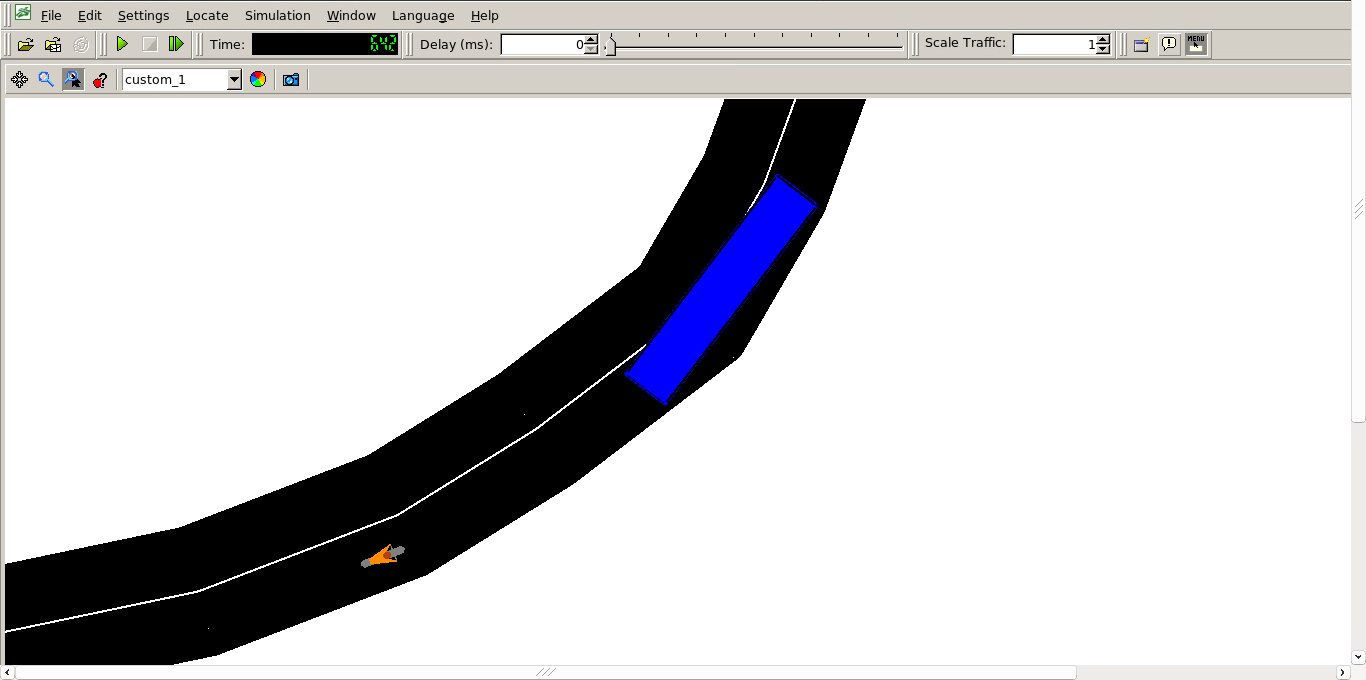
\includegraphics[width=\columnwidth]{captura2.png}
\caption{Moto con \texttt{speedMode 0} (naranja) a punto de embestir al bus11 en la
Vía Monay--Baguanchi--Paccha, $t=642$~s.}
\label{fig:moto}
\end{figure}

\subsection{Detección e inmovilización}
En cada paso se recorren las colisiones de \texttt{getCollisions()}. Si los tipos son
bus y moto, se registra un accidente \texttt{ACC\_nn} con su instante, tipo
(\emph{collision} o \emph{junction}), arista, posición y coordenadas; si el choque
ocurrió dentro de un cruce, la ambulancia se dirige a la siguiente arista de la ruta del
bus. Se dibuja un POI amarillo en el lugar y ambos vehículos se inmovilizan en dos pasos:
primero \texttt{speedMode 0} con velocidad 0 (se detienen en seco) y, en el paso
siguiente, \texttt{speedMode 31}, con lo que permanecen quietos sin generar frenadas de
emergencia. El resto de colisiones (de fondo) se resuelven retirando a los implicados
para que no bloqueen la vía.

\subsection{Despacho}
Cada accidente avanza por los estados \emph{espera} $\rightarrow$ \emph{en\_camino}
$\rightarrow$ \emph{atendiendo} $\rightarrow$ \emph{retorno} $\rightarrow$
\emph{cerrado}. Para despachar se calcula
\texttt{findRoute(hospital, accidente, vType="ambulance")} desde los siete hospitales y se
ordenan por \texttt{travelTime}. Se pide una unidad en ese orden y se acepta la primera
concedida, lo que equivale a elegir el hospital de menor tiempo de viaje entre los que
tienen stock y no la niegan. Si ninguno puede, el accidente sigue en espera y se
reintenta cada 30~s. Así ocurrió, por ejemplo, en ACC\_10: MUNI\_VALLE (139~s) negó la
unidad por el sorteo y VCM (211~s) no tenía stock, por lo que salió una unidad de
MONTE\_SINAI con un tiempo estimado de 323~s.

\subsection{Llegada}
La ambulancia se considera llegada si su distancia de conducción al accidente
(\texttt{getDistanceRoad}) es de 50~m o menos, si está detenida en la arista del
accidente, o si lleva 30~s detenida a menos de 300~m (el equipo sigue a pie). Mientras
está en camino se recalcula su ruta cada 60~s con \texttt{rerouteTraveltime}. Al llegar se
detiene con velocidad 0 y sin cambios de carril. La distancia no se mide mientras la
ambulancia está en un carril interno de un cruce, porque SUMO no admite posiciones sobre
esos carriles.

\subsection{Atención y retorno}
Tras 120~s de atención se retiran el bus, la moto y el POI, lo que libera la vía. Se
elige el hospital con menor \texttt{travelTime} desde el accidente, sin exigir que tenga
stock, y se devuelve el control a SUMO antes de cambiar el destino:
\begin{lstlisting}
def devolver_control(vid):
    # Krauss completo, LC2013 por defecto y
    # sin velocidad impuesta
    traci.vehicle.setSpeedMode(vid, 31)
    traci.vehicle.setLaneChangeMode(vid, 1621)
    traci.vehicle.setSpeed(vid, -1)

devolver_control(amb)
traci.vehicle.changeTarget(amb, hosp[hid]["edge"])
\end{lstlisting}
Sin restaurar el modo de cambio de carril, la ambulancia podría quedar en un carril sin
conexión con su nueva ruta. Cuando la ambulancia aparece en \texttt{getArrivedIDList}, la
unidad entra en la cola del hospital de retorno y el tiempo de la misión se suma al
hospital de origen. El stock de todos los hospitales se registra cada 60~s.

La Fig.~\ref{fig:accidente} muestra la secuencia completa sobre ACC\_06, en el Camino a
Turi: el bus y la moto inmovilizados en rojo, la cola que se forma detrás (los colores
indican el tiempo de espera) y la ambulancia acercándose. La Fig.~\ref{fig:retorno}
muestra la ambulancia ya incorporada al tráfico en su retorno, una vez retirados los
vehículos accidentados.

\begin{figure}[!t]
\centering
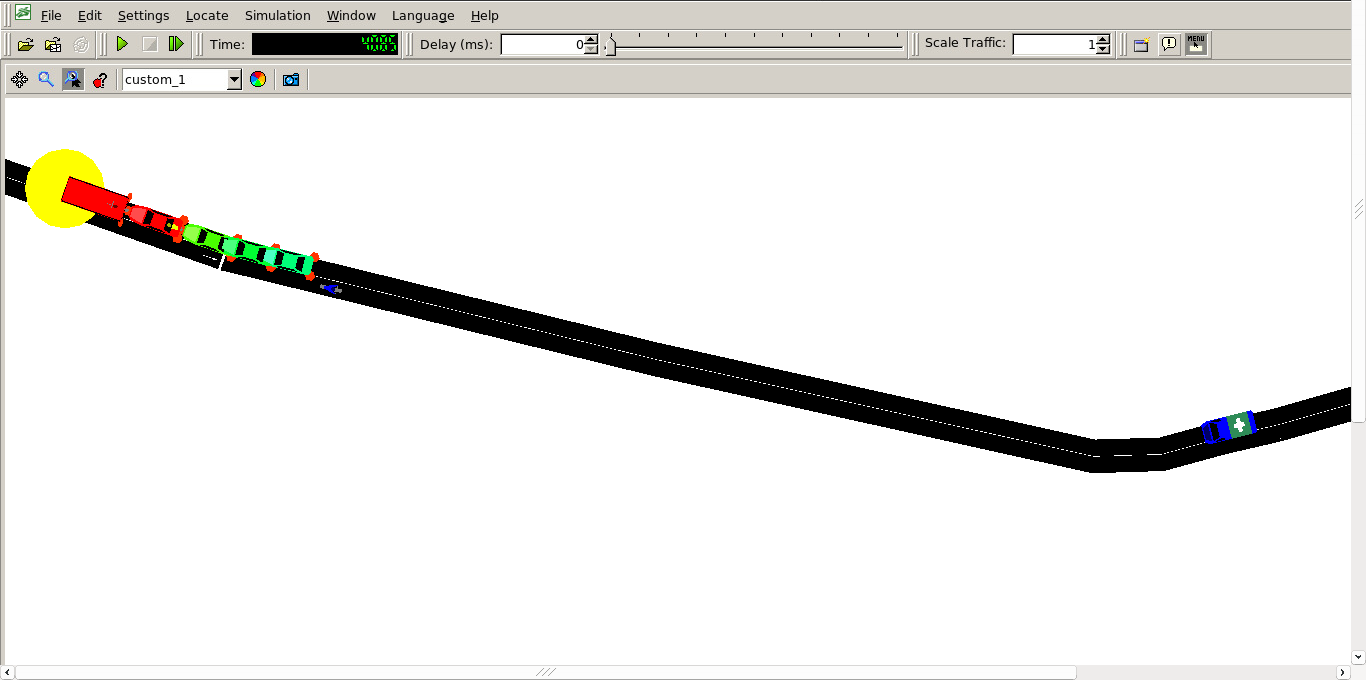
\includegraphics[width=\columnwidth]{RA_accidente_Teran.png}
\caption{ACC\_06 a $t\approx4085$~s: vehículos accidentados inmovilizados (rojo), cola
coloreada por tiempo de espera y ambulancia en camino (derecha).}
\label{fig:accidente}
\end{figure}

\begin{figure}[!t]
\centering
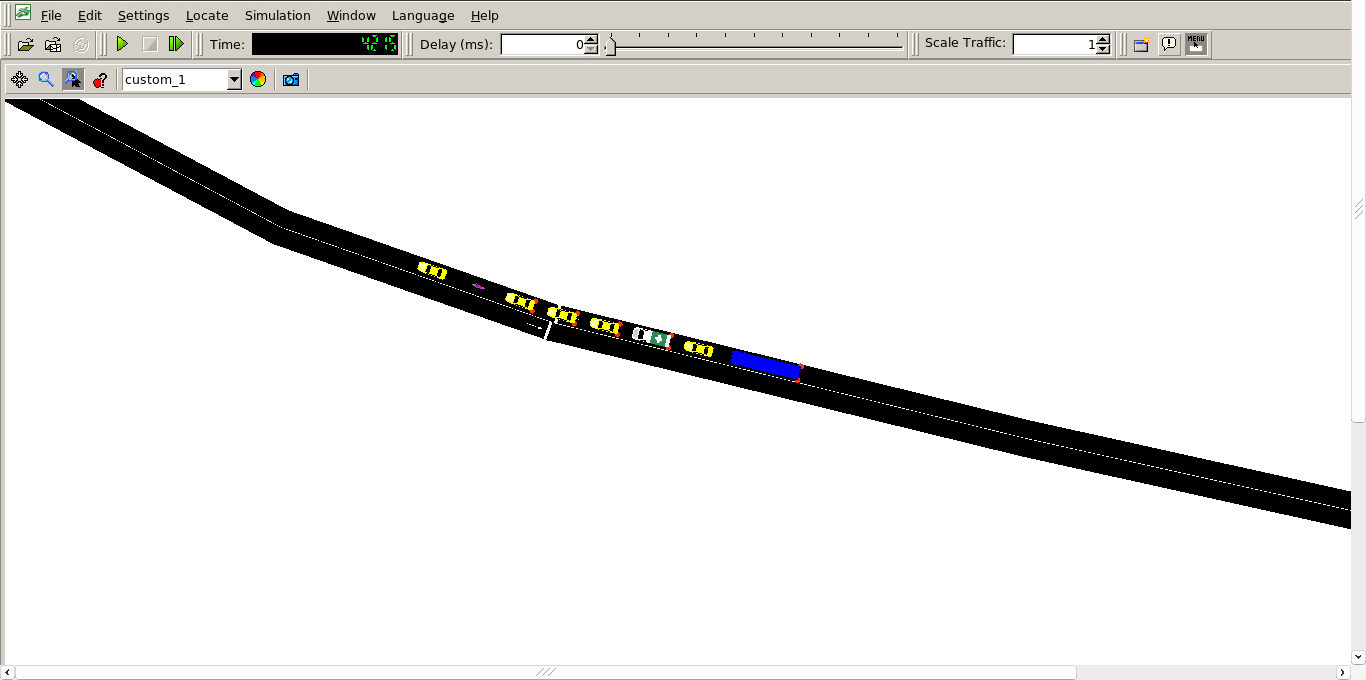
\includegraphics[width=\columnwidth]{captura5.png}
\caption{Tras la atención de ACC\_06 se retiran bus y moto; la ambulancia recupera el
control normal y regresa entre el tráfico.}
\label{fig:retorno}
\end{figure}

\subsection{Estadísticas}
Al cerrar TraCI se escriben \texttt{accidentes.csv} (todos los instantes de cada
accidente, origen, retorno y rutas), \texttt{hospitales.csv} (stock inicial y final,
despachos, retornos, negativas, tiempo ocupado y utilización) y \texttt{stock.csv}.
El script \texttt{analisis.py} calcula los indicadores con pandas, lee los totales de
\texttt{statistic-output} y genera las figuras con matplotlib; el mapa usa sumolib y
\texttt{convertXY2LonLat}. La utilización de un hospital se define como el tiempo de
misión de sus unidades dividido entre $3\,\mathrm{h}\times$ su stock inicial.

% ===========================================================================
\section{Resultados}
% ===========================================================================
\subsection{Accidentes sin atención (fase 3)}
Antes de añadir las ambulancias, la versión de la fase 3 produjo los 15 accidentes
previstos (5 por hora) en 15 aristas distintas, con dos intentos reprogramados y 0
teletransportes. Como nadie retiraba a los accidentados, al final de la corrida seguían
693 vehículos en la red y 30 no habían podido entrar, frente a un solo vehículo en la
corrida de referencia. La Fig.~\ref{fig:atasco} muestra la cola detrás de ACC\_06 casi
dos horas después del choque: unos 43 vehículos detenidos en una vía de un carril. Las
estadísticas de viaje de esa corrida (tiempo perdido medio de 125~s) parecen mejores que
las de referencia solo porque promedian los 4094 viajes completados y excluyen a los
vehículos atrapados.

\begin{figure}[!t]
\centering
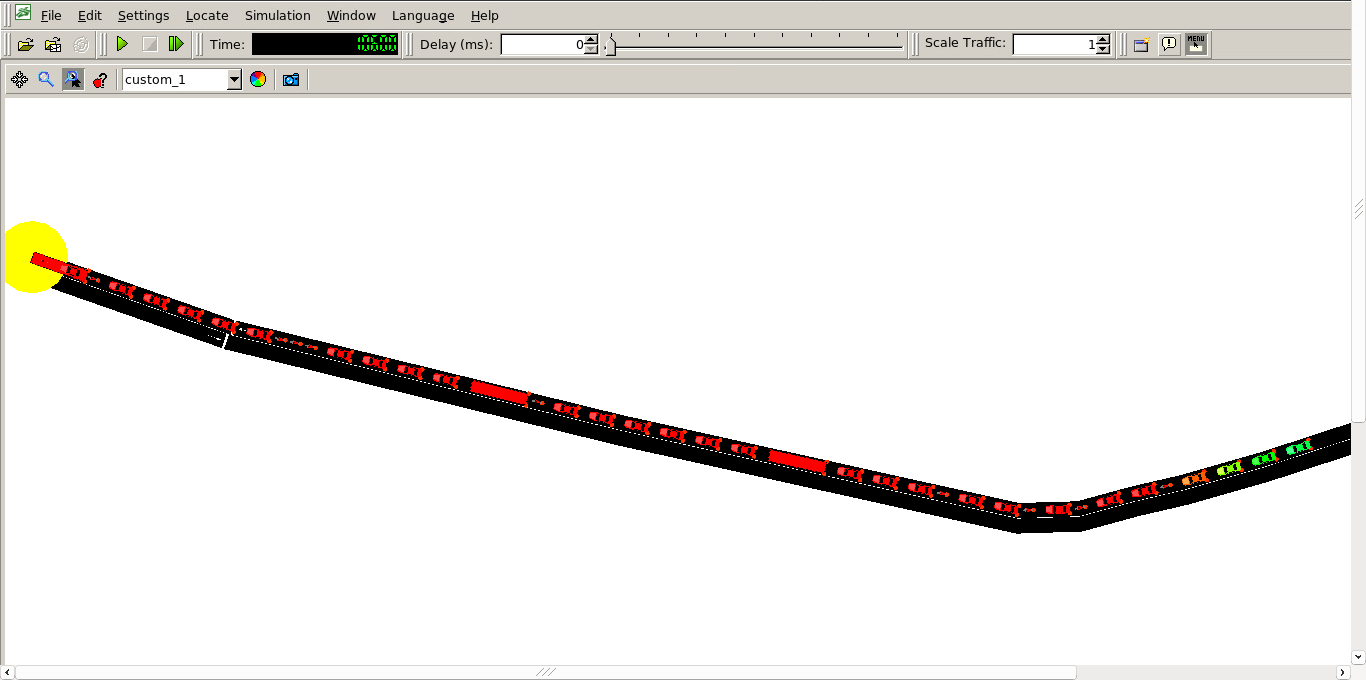
\includegraphics[width=\columnwidth]{captura3.png}
\caption{Fase 3 sin ambulancias, $t=10\,600$~s: la cola detrás de ACC\_06 (POI
amarillo) se extiende por toda la vía; rojo indica mayor tiempo de espera.}
\label{fig:atasco}
\end{figure}

\subsection{Corrida completa (fases 4 y 5)}
La Tabla~\ref{tab:registro} resume la corrida completa y la Tabla~\ref{tab:acc} detalla
cada accidente. Los 15 accidentes terminaron en estado \emph{cerrado}, al final de la
simulación quedaban tres vehículos en la red y no hubo teletransportes. De las 23
colisiones, 15 son los accidentes provocados y 8 son colisiones espontáneas de fondo,
cuyos 16 vehículos se retiraron. Las 84 paradas de emergencia que reporta SUMO
corresponden a una sola moto de un intento abortado que, con el cambio de carril
desactivado, quedó en un carril sin conexión con su siguiente arista hasta que recuperó
el control.

\begin{table}[!t]
\centering
\caption{Registro de la corrida completa (3~h de demanda, semilla 42)}
\label{tab:registro}
\footnotesize
\begin{tabular}{@{}p{0.58\columnwidth}r@{}}
\toprule
Magnitud & Valor \\
\midrule
Aristas / semáforos de la red & 1501 / 98 \\
Vehículos de fondo (car / bus / moto) & 3600 / 300 / 900 \\
Insertados por TraCI (motos / ambulancias) & 15 / 16 \\
Teleports / colisiones / colisiones bus--moto & 0 / 23 / 15 \\
Accidentes registrados (h1 / h2 / h3) & 15 (5 / 5 / 5) \\
Flota inicial (públicos / privados) & 10 / 0 \\
Respuesta: mediana / media / p90 / máx (s) & 265 / 233,7 / 353,8 / 364 \\
Accidentes con espera / espera máx. (s) & 0 / 0 \\
Retornos a un hospital distinto del de origen & 7 de 15 (47\,\%) \\
Tiempo de pared de la corrida (s) & 40,0 \\
\bottomrule
\end{tabular}
\end{table}

\begin{table}[!t]
\centering
\caption{Accidentes atendidos (tiempos en segundos)}
\label{tab:acc}
\footnotesize
\setlength{\tabcolsep}{3.5pt}
\begin{tabular}{@{}lrlrrlr@{}}
\toprule
Acc. & $t_{\mathrm{acc}}$ & Origen & Resp. & ETA & Retorno & Misión \\
\midrule
01 & 645  & MUNI\_VALLE  & 86  & 108 & MUNI\_VALLE  & 428 \\
02 & 764  & VCM          & 120 & 130 & MILITAR      & 420 \\
03 & 2109 & VCM          & 311 & 338 & MONTE\_SINAI & 858 \\
04 & 2407 & MILITAR      & 124 & 146 & MILITAR      & 312 \\
05 & 2762 & MUNI\_VALLE  & 333 & 273 & IESS\_JCA    & 510 \\
06 & 3751 & MONTE\_SINAI & 343 & 270 & MONTE\_SINAI & 686 \\
07 & 3944 & MILITAR      & 210 & 183 & MONTE\_SINAI & 442 \\
08 & 4451 & MUNI\_PAT    & 146 & 121 & MUNI\_PAT    & 340 \\
09 & 5630 & MUNI\_PAT    & 364 & 205 & MUNI\_PAT    & 650 \\
10 & 5771 & MONTE\_SINAI & 361 & 323 & IESS\_JCA    & 819 \\
11 & 8208 & MUNI\_PAT    & 280 & 210 & MUNI\_PAT    & 680 \\
12 & 8717 & MILITAR      & 170 & 181 & MONTE\_SINAI & 361 \\
13 & 8824 & MONTE\_SINAI & 313 & 264 & MUNI\_PAT    & 831 \\
14 & 9735 & MUNI\_PAT    & 265 & 206 & MUNI\_PAT    & 571 \\
15 & 9784 & MONTE\_SINAI & 80  & 84  & MONTE\_SINAI & 233 \\
\bottomrule
\end{tabular}
\end{table}

Como ningún accidente esperó, el tiempo total desde el choque hasta la llegada coincide
con el tiempo de respuesta. La duración de las misiones tuvo una mediana de 510~s y un
p90 de 826~s. La Fig.~\ref{fig:respuesta} muestra la respuesta de cada accidente. En
varios casos la respuesta real supera con claridad a la estimación de \texttt{findRoute}
(ACC\_09: 364~s frente a 205~s), porque la estimación usa los tiempos de viaje del
momento del despacho y no anticipa la cola que genera el propio accidente.

\begin{figure}[!t]
\centering
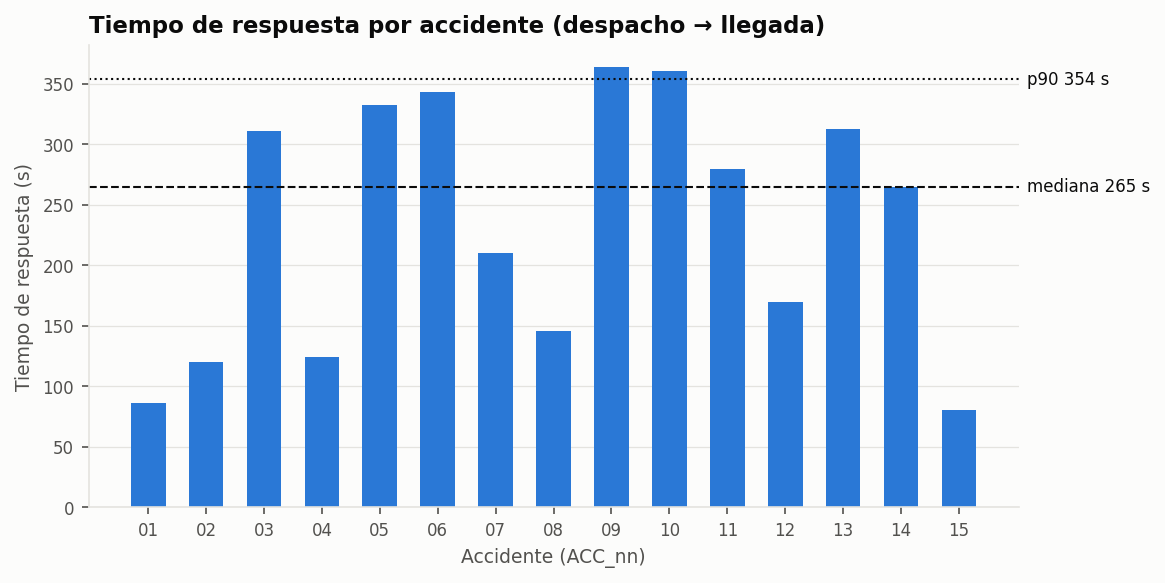
\includegraphics[width=\columnwidth]{RA_fig_a_respuesta.png}
\caption{Tiempo de respuesta (despacho $\rightarrow$ llegada) por accidente, con su
mediana y su p90.}
\label{fig:respuesta}
\end{figure}

\subsection{Uso de la flota}
La Tabla~\ref{tab:hosp} y la Fig.~\ref{fig:hosp} resumen el uso de cada hospital, y la
Fig.~\ref{fig:stock} su stock a lo largo del tiempo. VCM terminó sin unidades a pesar de
empezar con tres: despachó dos y una tercera fue la ambulancia de prueba, que quedó en
IESS\_JCA, y ninguna volvió. MONTE\_SINAI, sin stock inicial, terminó despachando cuatro
unidades gracias a los retornos que recibió. MILITAR fue el hospital público más usado,
con una utilización del 10,3\,\%.

\begin{table}[!t]
\centering
\caption{Uso de ambulancias por hospital}
\label{tab:hosp}
\footnotesize
\setlength{\tabcolsep}{3pt}
\begin{tabular}{@{}llrrrrrr@{}}
\toprule
Hospital & Tipo & Ini. & Fin & Desp. & Ret. & Rech. & Util. \\
\midrule
VCM          & público & 3 & 0 & 2 & 0 & 0 & 3,9\,\% \\
IESS\_JCA    & público & 1 & 4 & 0 & 2 & 0 & 0,0\,\% \\
MILITAR      & público & 1 & 0 & 3 & 2 & 0 & 10,3\,\% \\
MUNI\_PAT    & público & 3 & 4 & 4 & 5 & 0 & 6,9\,\% \\
MUNI\_VALLE  & público & 2 & 1 & 2 & 1 & 1 & 4,3\,\% \\
MONTE\_SINAI & privado & 0 & 1 & 4 & 5 & 1 & n/a \\
DEL\_RIO     & privado & 0 & 0 & 0 & 0 & 0 & n/a \\
\bottomrule
\end{tabular}
\\[2pt]
\parbox{\columnwidth}{\scriptsize Rech.: negativas por $p_{\mathrm{sin}}$. Las veces
que un hospital fue consultado sin stock fueron VCM 4, MONTE\_SINAI 3 y DEL\_RIO 3. El
stock de IESS\_JCA incluye la unidad de prueba procedente de VCM.}
\end{table}

\begin{figure}[!t]
\centering
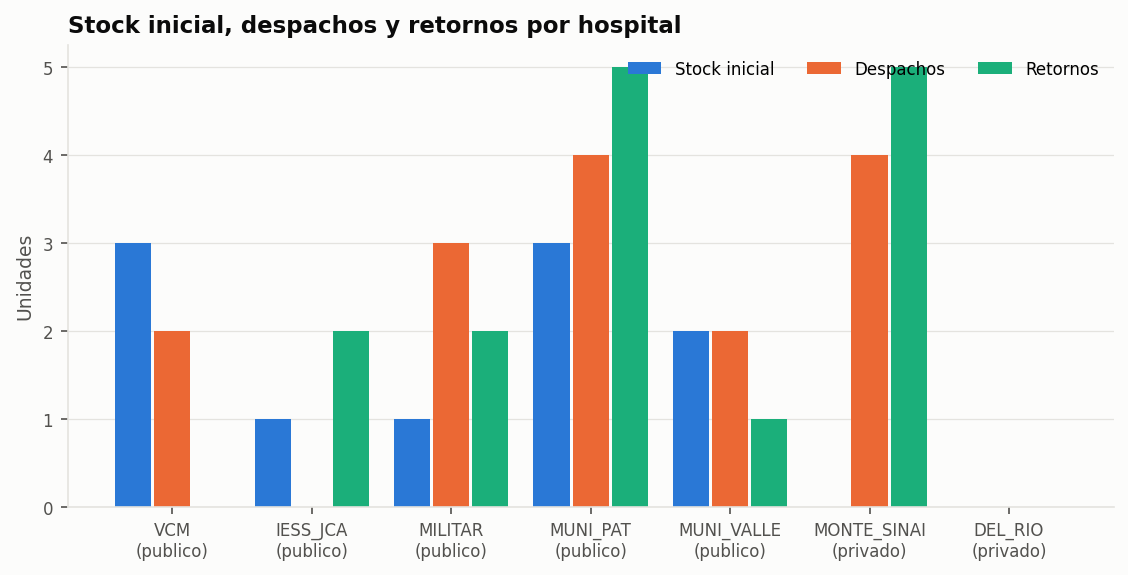
\includegraphics[width=\columnwidth]{RA_fig_b_hospitales.png}
\caption{Stock inicial, despachos y retornos por hospital.}
\label{fig:hosp}
\end{figure}

\begin{figure*}[!t]
\centering
\begin{minipage}[t]{0.40\textwidth}
\centering
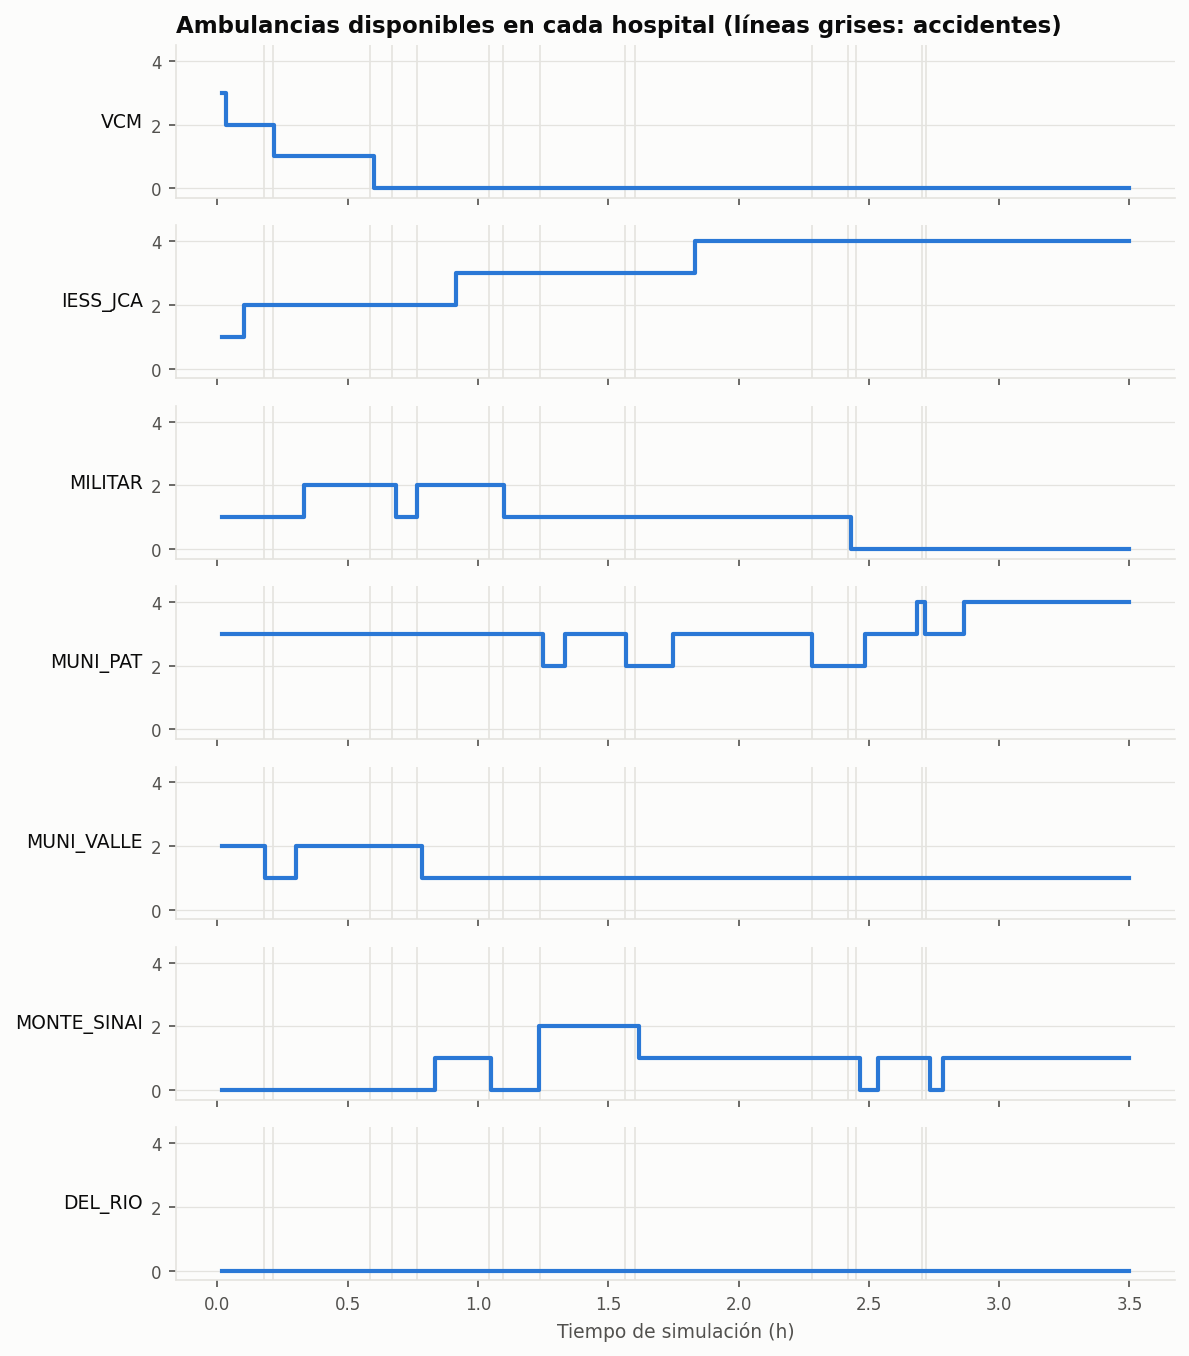
\includegraphics[width=\textwidth]{RA_fig_c_stock.png}
\caption{Ambulancias disponibles en cada hospital (las líneas grises marcan los
accidentes).}
\label{fig:stock}
\end{minipage}\hfill
\begin{minipage}[t]{0.57\textwidth}
\centering
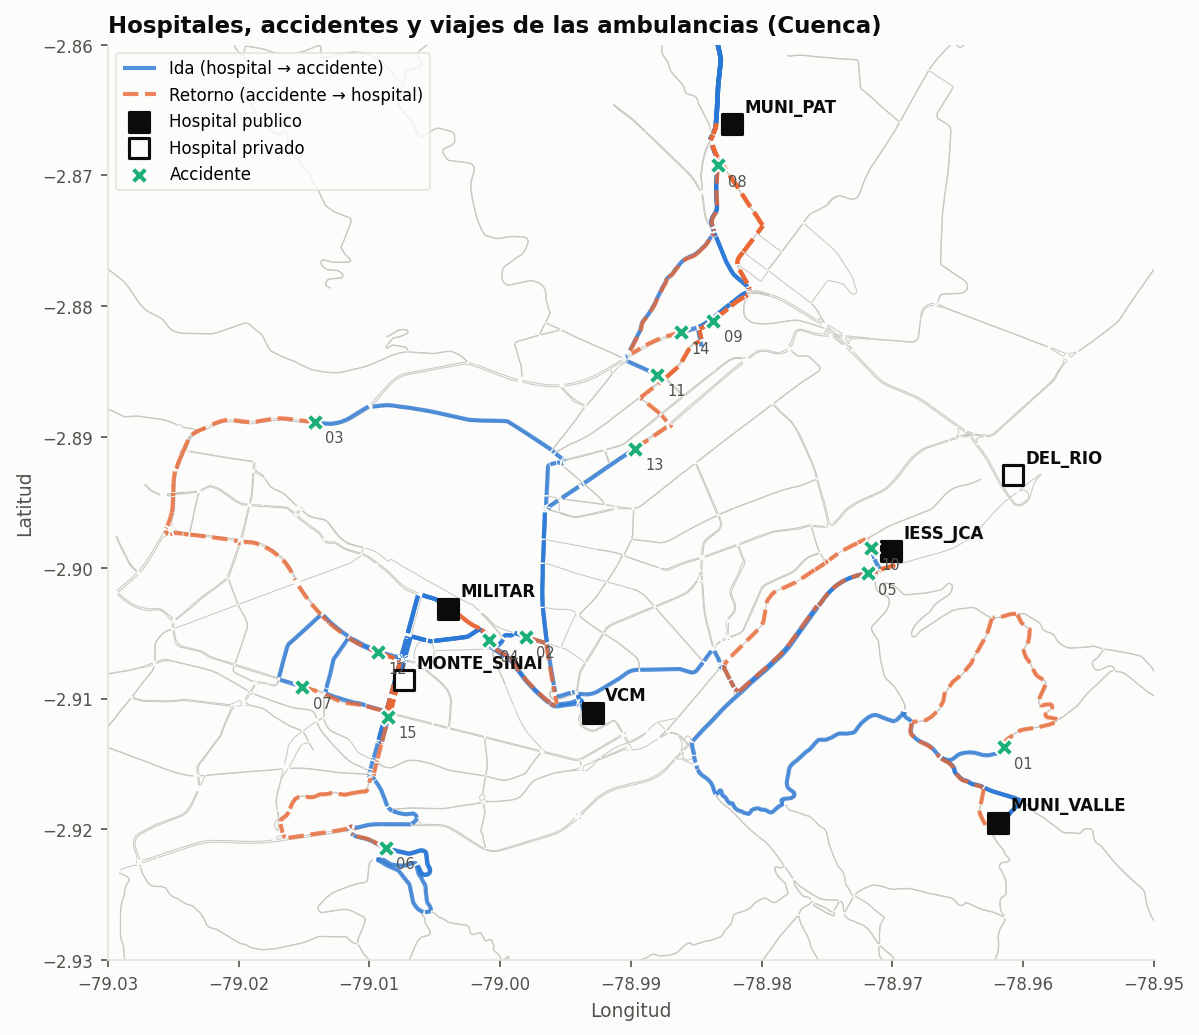
\includegraphics[width=\textwidth]{RA_fig_d_mapa.png}
\caption{Red, hospitales (cuadrados), accidentes (cruces) y viajes de ida (azul) y
retorno (naranja discontinuo).}
\label{fig:mapa}
\end{minipage}
\end{figure*}

La Fig.~\ref{fig:mapa} sitúa los accidentes y los viajes sobre la red, y la
Fig.~\ref{fig:red} muestra la red en sumo-gui con los POI de los hospitales (verde:
públicos, azul: privados).

\begin{figure}[!t]
\centering
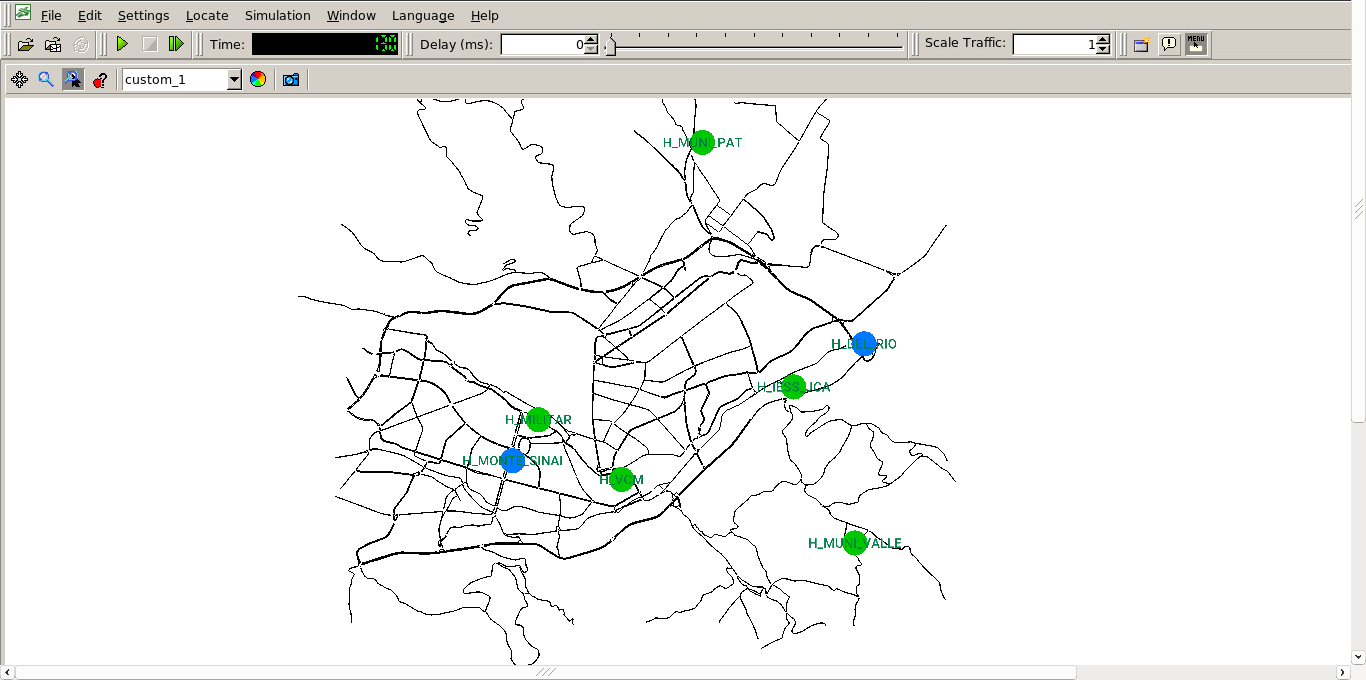
\includegraphics[width=\columnwidth]{captura4.png}
\caption{Red \texttt{cuenca\_ciudad} en sumo-gui con los siete hospitales.}
\label{fig:red}
\end{figure}

% ===========================================================================
\section{Análisis}
% ===========================================================================
\subsection{Colisión imposible}
Mientras el bit~0 de \texttt{speedMode} está activo, la moto aplica
$v=\min(v_{\mathrm{safe}},v_{\max},v+a\Delta t)$ y frena detrás del bus aunque
\texttt{setSpeed(22)} eleve $v_{\max}$: la orden de TraCI solo modifica uno de los
términos del mínimo. Con \texttt{setSpeedMode(0)}, $v_{\mathrm{safe}}$ desaparece y la moto
alcanza al bus a 22~m/s. Con \texttt{setSpeedMode(30)} (todos los bits salvo el 0) el
choque también se produciría, porque sigue faltando $v_{\mathrm{safe}}$; la única
diferencia es que la moto respetaría sus límites de aceleración y desaceleración, de modo
que tardaría algo más en llegar a 22~m/s. Con \texttt{setSpeedMode(23)} (todos salvo el
bit~3) $v_{\mathrm{safe}}$ sigue activa y no habría choque por alcance; la moto solo
ignoraría la prioridad en los cruces, por lo que podría chocar lateralmente con otro
vehículo en una intersección, pero no con el bus que la precede.

\subsection{Teletransportes y acción de colisión}
Con \texttt{time-to-teleport} en su valor por defecto (300~s), los vehículos detenidos
detrás del accidente saltarían por delante de él tras 5~min, el bus y la moto
inmovilizados también serían teletransportados y la cola desaparecería. El reto mediría
entonces un tráfico casi normal: la duración media, el tiempo perdido, el tiempo de
espera y el número de vehículos en marcha al final serían falsamente bajos, y la
ambulancia encontraría una vía libre, con tiempos de respuesta optimistas. Con
\texttt{collision.action} en su valor por defecto (\emph{teleport}), los vehículos
implicados desaparecerían de su carril en el instante del choque. No quedaría ningún
accidente que inmovilizar ni que atender, la ambulancia se dirigiría a un lugar vacío y el
número de teletransportes ya no mediría bloqueos sino colisiones.

\subsection{Tiempo frente a distancia}
ACC\_10 ocurrió en la avenida José Carrasco Arteaga, a solo 174~m en línea recta del
hospital IESS\_JCA, que en ese momento tenía tres unidades. Sin embargo, IESS\_JCA ni
siquiera fue consultado antes que MONTE\_SINAI, a 4,1~km en línea recta: su arista de
salida está sobre la Circunvalación Sur y apunta en sentido contrario al accidente, y como
la red no permite giros en U fuera de las calles sin salida, la ruta debe dar un largo
rodeo. En flujo libre, la ruta más rápida desde IESS\_JCA hasta el
accidente recorre 9,4~km y tarda unos 567~s, mientras que desde MUNI\_VALLE son 3,2~km
(164~s). El sorteo descartó a MUNI\_VALLE y VCM no tenía stock, por lo que salió
MONTE\_SINAI (323~s). ACC\_03 ilustra lo mismo: VCM, el más lejano de los tres
hospitales más cercanos en línea recta (3,4~km), fue el elegido porque la avenida de las
Américas permite llegar en menos tiempo que desde MILITAR, situado en el centro con calles
lentas y semaforizadas. El \texttt{travelTime} recoge el sentido de las vías, la
velocidad permitida y la congestión del momento; la distancia en línea recta no recoge
ninguno de estos factores.

\subsection{Disponibilidad aleatoria}
En $t=0$ los cinco hospitales públicos tienen stock y los privados no tienen ninguno, de
modo que ningún hospital puede atender solo si los cinco públicos niegan la unidad:
\begin{equation}
P = p_{\mathrm{sin}}^{5} = 0{,}25^{5} \approx 9{,}8\times10^{-4} \approx 0{,}1\text{\,\%}.
\end{equation}
Durante la corrida, VCM y MILITAR se vaciaron. Incluso con solo tres hospitales con stock,
la probabilidad sería $0{,}25^{3}\approx1{,}6\text{\,\%}$, y MONTE\_SINAI añadía unidades
procedentes de los retornos. El número esperado de accidentes en espera en 15 sorteos es
inferior a 0,25, coherente con la fracción observada de 0 de 15. La negativa aleatoria
retrasó varios despachos (ACC\_10, ACC\_12), pero no dejó ningún accidente sin
ambulancia.

\subsection{Redistribución de la flota}
Según \texttt{stock.csv}, VCM se vació a los 36~min y MILITAR en la tercera hora. Ambos
están en el centro y oeste, donde ocurrieron la mayoría de los accidentes. Sin embargo,
el hospital más cercano a esos lugares es a menudo MILITAR o MONTE\_SINAI, por lo que las
unidades de VCM no volvieron a él. IESS\_JCA acumuló cuatro unidades sin despachar
ninguna: es muy accesible para llegar desde el este (recibió los retornos de ACC\_05 y
ACC\_10) pero muy lento para salir, por el efecto descrito en el caso de ACC\_10.
MUNI\_PAT también acumuló cuatro, porque atendió y recibió de vuelta los accidentes del
norte. En consecuencia, la flota se desplaza hacia hospitales periféricos con buena
accesibilidad de entrada y se vacía en los centrales.

\subsection{Utilización}
Las misiones sumaron 8141~s frente a una capacidad de $10\times10\,800=108\,000$~s, una
utilización global del 7,5\,\%. Es baja porque hay pocas emergencias para la flota
disponible: 15 accidentes de unos 9~min cada uno ocupan en promedio menos de una de las
diez unidades. La tasa de accidentes no es extrema, y la utilización máxima (MILITAR,
10,3\,\%) se debe a que solo tenía una unidad inicial. Con 15 accidentes por hora habría
unas 45 misiones y, con la misma duración, la utilización global se acercaría al 23\,\%.
Sin embargo, el efecto no sería lineal: más accidentes generan más congestión y misiones
más largas, los hospitales centrales se vaciarían antes y empezarían a aparecer esperas
por falta de ambulancia.

% ===========================================================================
\section{Extensión: política de retorno}
% ===========================================================================
Se añadió al script la opción \texttt{--retorno origen}, con la que cada ambulancia vuelve
a su hospital de origen en lugar de al más cercano al accidente; las salidas se escriben
en otra carpeta y \texttt{comparar.py} contrasta ambas corridas (Tabla~\ref{tab:ext} y
Fig.~\ref{fig:ext}). Como las ambulancias alteran el tráfico, las dos corridas no son
idénticas: con la política de origen se registraron 17 accidentes, porque dos colisiones
espontáneas bus--moto en cruces se contabilizaron como accidentes, y los buses elegidos por
la agenda difieren. La tabla incluye también las cifras restringidas a los 15 accidentes
de la agenda.

\begin{table}[!t]
\centering
\caption{Comparación de las políticas de retorno (tiempos en segundos)}
\label{tab:ext}
\footnotesize
\setlength{\tabcolsep}{4pt}
\begin{tabular}{@{}lrr@{}}
\toprule
 & Más cercano & Origen \\
\midrule
Accidentes (todos / de la agenda) & 15 / 15 & 17 / 15 \\
Respuesta: mediana & 265 & 214 \\
Respuesta: media & 233,7 & 259,9 (266,8) \\
Respuesta: p90 & 353,8 & 437,8 (486,2) \\
Respuesta: máxima & 364 & 675 \\
Misión: mediana & 510 & 675 \\
Público más usado & MILITAR 10,3\,\% & MILITAR 40,6\,\% \\
Consultas a privados sin stock & 6 & 13 \\
Vehículos en la red al final & 3 & 14 \\
\bottomrule
\end{tabular}
\\[2pt]
\parbox{\columnwidth}{\scriptsize Entre paréntesis: solo los 15 accidentes de la agenda.}
\end{table}

\begin{figure*}[!t]
\centering
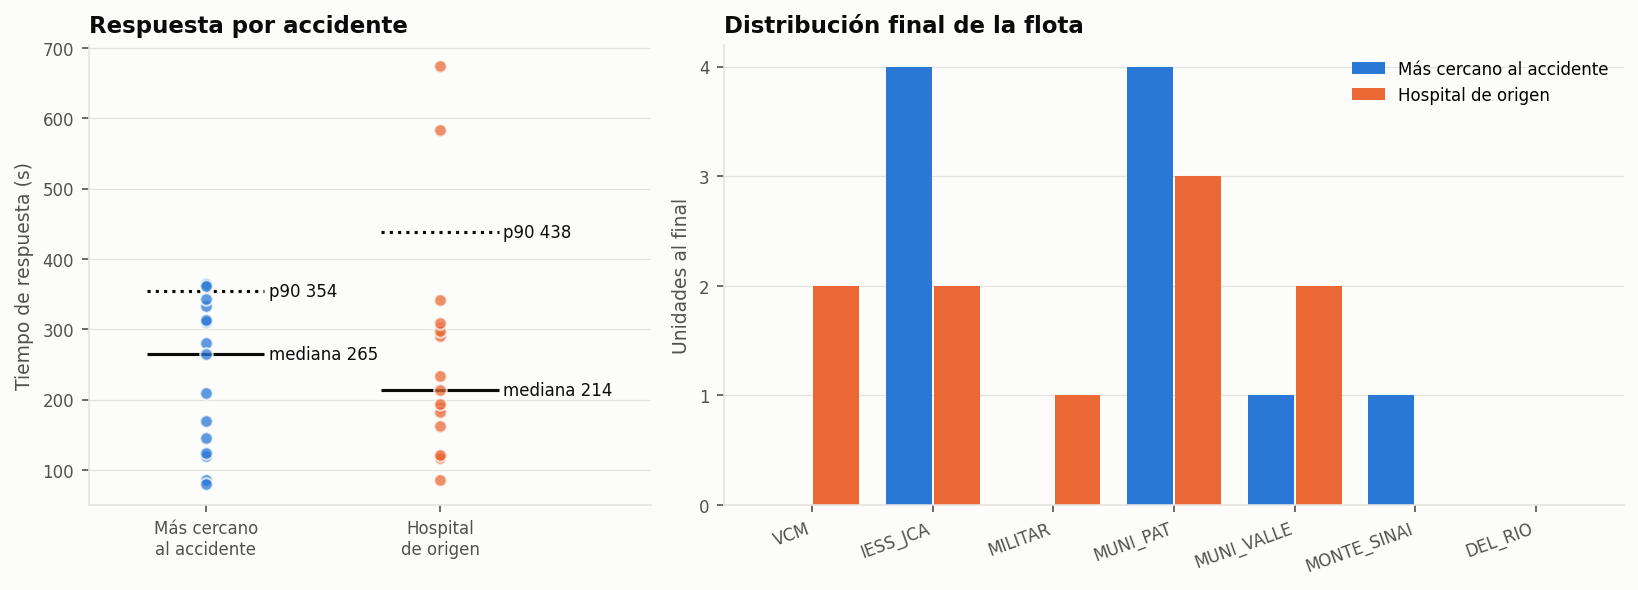
\includegraphics[width=0.72\textwidth]{RA_fig_e_extension.png}
\caption{Extensión: tiempo de respuesta por accidente y distribución final de la flota
según la política de retorno.}
\label{fig:ext}
\end{figure*}

Volver al hospital de origen conserva la distribución inicial de la flota (cada hospital
termina con las mismas unidades, salvo la de prueba) y logra una mediana de respuesta algo
menor. Sin embargo, alarga las misiones, porque la ambulancia regresa a un hospital que
puede estar lejos del accidente; eso mantiene ocupada más tiempo a la unidad y empeora la
cola de la distribución: el p90 pasa de 354 a 438~s y el máximo de 364 a 675~s. Además,
los hospitales privados nunca reciben unidades, de modo que la carga se concentra en
MILITAR, cuya única unidad estuvo ocupada el 40,6\,\% del tiempo. Con un solo par de
corridas las diferencias de mediana no son concluyentes, pero las del p90, el máximo y
la duración de misión son grandes y consistentes con el mecanismo descrito.

% ===========================================================================
\section{Discusión}
% ===========================================================================
\textbf{Calibración del gemelo.} Harían falta los registros del ECU~911 con la hora, el
lugar y el tipo de cada accidente para sustituir la agenda uniforme; la flota real por
hospital y sus turnos; los tiempos reales de atención en el sitio y de traslado del
paciente; y conteos de tráfico o matrices origen--destino para calibrar la demanda, que
hoy es aleatoria. Los supuestos que más cambiarían los resultados son el tiempo de
atención (120~s es muy inferior a una atención real y omite el traslado al hospital, que
multiplicaría la duración de las misiones y la utilización), el stock inicial con
$p_{\mathrm{sin}}$, y la ausencia de prioridad para la ambulancia, que hoy respeta
semáforos y cruces como cualquier vehículo.

\textbf{El equipo sigue a pie.} El criterio de 30~s detenida a menos de 300~m sustituye a lo que en la
realidad hacen los conductores al oír la sirena: abrir un corredor de emergencia. En SUMO
este comportamiento se modela con el dispositivo \emph{bluelight}, que hace que los
vehículos cercanos se aparten y permite a la ambulancia cruzar en rojo, junto con el
modelo de subcarriles para que los vehículos se desplacen lateralmente. Con V2X, la
ambulancia difundiría mensajes CAM o DENM (como en ms-van3t, temas de las clases 8 a 10);
los vehículos que los reciban dentro de cierto radio y por delante de ella se podrían
mover con TraCI mediante \texttt{changeLane} o \texttt{slowDown}, o bien pasando al lado
de la calzada.

\textbf{Política de retorno.} Con las cifras de la extensión, el retorno al hospital más
cercano al accidente conviene más a la ciudad: acorta la mediana de las misiones en un
24\,\% (de 675 a 510~s), reduce el p90 de la respuesta de 438 a 354~s y reparte la carga
entre más hospitales, incluidos los privados. Su desventaja es que vacía los hospitales
centrales, como VCM. Una política mixta, con retorno al más cercano y un reequilibrio
periódico de unidades hacia los hospitales vacíos, combinaría ambas ventajas.

% ===========================================================================
\section{Conclusiones}
% ===========================================================================
\begin{itemize}
\item El término $v_{\mathrm{safe}}$ de Krauss es lo único que hace imposibles los choques
en SUMO. Al apagar el bit~0 de \texttt{speedMode} en una moto se provocaron 15 accidentes
reproducibles, cinco por hora y en lugares distintos.
\item \texttt{time-to-teleport = -1} y \texttt{collision.action = warn} son
imprescindibles: sin ellos los accidentes y sus colas desaparecen, y las estadísticas
dejan de reflejar el bloqueo. La fase 3 mostró que un accidente sin atender bloquea la
red hasta el final (693 vehículos atrapados).
\item El despacho por \texttt{travelTime} elige hospitales que no son los más cercanos en
línea recta, sobre todo cuando el sentido de las vías obliga a dar rodeos (IESS\_JCA). La
respuesta tuvo una mediana de 265~s y un p90 de 354~s.
\item Con 10 unidades y 5 accidentes por hora, la flota se usa poco (7,5\,\% global) y
ningún accidente esperó; el retorno al hospital más cercano redistribuye la flota hacia la
periferia, pero ofrece mejores colas de respuesta que el retorno al origen.
\end{itemize}

\textbf{Dificultades encontradas.} El contenedor del curso incluía SUMO~1.12 sin TraCI
para Python, por lo que se instaló SUMO~1.28 con \texttt{pip --target} en la carpeta
compartida. La API de OpenStreetMap obligó a descargar el área en 25 teselas. Un cuello de
botella en Barrial Blanco dejaba vehículos atrapados hasta que se activó el rerouting.
\texttt{getStartingTeleportNumber} cuenta solo los teletransportes de cada paso y hubo que
acumularlo. \texttt{getDistanceRoad} falla sobre los carriles internos de los cruces.
Por último, una moto con el cambio de carril desactivado puede quedar atrapada en un carril
sin salida.

\textbf{Sugerencias.} Distribuir el contenedor con SUMO~1.28 y TraCI ya instalados, y el
archivo OSM del área ya descargado. Aclarar en las láminas que \texttt{setSpeed} no
desactiva el modelo de seguimiento (solo lo hace \texttt{setSpeedMode}). Pedir varias
semillas por política para que las comparaciones tengan intervalos de confianza.

% ===========================================================================
\begin{thebibliography}{9}
\bibitem{sumo} P.~A. Lopez \emph{et al.}, ``Microscopic traffic simulation using SUMO,''
in \emph{Proc. IEEE 21st Int. Conf. Intelligent Transportation Systems (ITSC)}, 2018,
pp. 2575--2582.
\bibitem{krauss} S.~Krauß, ``Microscopic modeling of traffic flow: Investigation of
collision free vehicle dynamics,'' Ph.D. dissertation, Univ. of Cologne, 1998.
\bibitem{traci} SUMO, ``TraCI/Change Vehicle State,'' [Online]. Available:
\url{https://sumo.dlr.de/docs/TraCI/Change_Vehicle_State.html}
\bibitem{vtypedef} SUMO, ``Vehicle Type Parameter Defaults,'' 2024. [Online]. Available:
\url{https://sumo.dlr.de/docs/Vehicle_Type_Parameter_Defaults.html}
\bibitem{osm} OpenStreetMap contributors, ``OpenStreetMap,'' [Online]. Available:
\url{https://www.openstreetmap.org}
\bibitem{vanet} ms-van3t developers, ``ms-van3t: A multi-stack V2X simulation and
emulation framework based on ns-3 and SUMO,'' 2024. [Online]. Available:
\url{https://github.com/ms-van3t-devs/ms-van3t}
\end{thebibliography}

% ===========================================================================
\appendix[Repositorio de entregables]
% ===========================================================================
La carpeta \texttt{reto/} con la red, \texttt{vtypes.add.xml}, los tres archivos
\texttt{.rou.xml}, \texttt{reto.sumocfg}, \texttt{reto\_ambulancias.py},
\texttt{analisis.py}, \texttt{comparar.py}, los CSV, los gráficos, las capturas y el
registro de eventos está disponible en:

\begin{center}
\url{https://github.com/USUARIO/REPOSITORIO}
\end{center}

\end{document}
